%\chapter{Background}  \label{background}
\chapter{Background}  \label{background}
%The syntax of a programming language describes its structure, and t
The structure of a program can be described using its syntax and a Java source code can be represented as an instance of an Abstract Syntax Tree. To construct structural generalizations describing the correspondences and differences between logged Java classes, first we should understand what AST is and how specific information about each Java element is held in AST structure. Then we should investigate the application of anti-unification and its extensions on this structure to produce structural generalizations. We should also figure out how the Jigsaw framework could assist us in determining potential candidate structural correspondences.

Anti-unification is summarized in section~\ref{AU} starting with an introduction to unification and its dual anti-unification and followed by a discourse regarding to limitations of anti-unification to address our problem. 
Sections~\ref{AST} and~\ref{AUAST} of this chapter establish a brief description of the Abstract Syntax Tree (AST) structure and its extended form, necessary to understand the requirements that guided the development of an anti-unification algorithm for our application.
Section~\ref{HOAUMT} is dedicated to explain higher-order anti-unification modulo theories, an extension to anti-unification, in which a set of equivalence theories are defined and applied on higher-order extended structures to incorporate background knowledge. 
Afterwards we discuss the Jigsaw framework and its application in determining potential candidate structural correspondences in Section~\ref{Jigsaw}.

\section{Anti-unification}   \label{AU}

To describe unification theory and its dual anti-unification theory, we first introduce a formal definition of term, the application of a substitution on a term, and the definition of instance and anti-instance of a term, as the requirements needed to understand the theories. 

\begin{defn}[Term]\label{def:term} 
A term is a set of function symbols, variables, and constants, such that function symbols can come up with unlimited number of arguments. 
\end{defn}

In the definition of a term, function symbols are represented by identifiers starting with a lowercase letter (e.g., \vars{f(a,b)}), variables are represented by identifiers starting with an uppercase letter (e.g., \vars{X}, \vars{Y}), and constants are function symbols with no arguments (e.g., \vars{a}, \vars{b}). the followings are examples of term:
\begin{itemize} [leftmargin=0.7in]
\item \vars{Y}
\item \vars{a}
\item \vars{f(X, c)}
\item \vars{f(g(X, b),Y, g(a, Z))}
\end{itemize}
%A term is called grounded if it does not contain any variables (e.g., \vars{f(a,b)}), and 
\begin{defn}[Applying substitutions]\label{def:substitution} 
A substitution is a mapping from variables to terms, and the application of a substitution to a term would result in replacing all occurrences of each variable in the term by a proper subterm.
\end{defn}

As an example, an application of a substitution $\ominus$ =
\begin{tikzcd}[column sep=small] \vars{X} \arrow[r,->,shift right,""] & \vars{a} \end{tikzcd}
 on a term \vars{f(X,b)} is defined by replacing all occurrences of the variable \vars{X} by the term \vars{a} and thus\begin{tikzcd}[column sep=small] \vars{f(X,b)} \arrow[r,->,shift right,"\ominus"] & \vars{f(a,b)} \end{tikzcd}.


\begin{defn}[instance \& anti-instance]\label{def:instance} 
 \vars{a} is an instance of a term \vars{X} and \vars{X} is an anti-instance of \vars{a}, if there is a substitution $\ominus$ such that the application of $\ominus$ on \vars{X} results in \vars{a} (\begin{tikzcd}[column sep=small]\vars{X} \arrow[r,->,shift right,"\ominus"] & \vars{a}\end{tikzcd}).
\end{defn} 

\begin{defn}[Unifier]\label{def:unifier} 
An unifier is a common instance of two given terms.
\end{defn} 

Unification usually aims to create the Most General Unifier (MGU), that is, \vars{U} is MGU of two terms such that for all unifiers \vars{U}${\prime}$ there exist a substitution $\ominus$ such that \begin{tikzcd}[column sep=small] \vars{U} \arrow[r,->,shift right,"\ominus"] & \vars{U$\prime$} \end{tikzcd}. Unification has been used for various applications, however, it is not helpful to solve our problem as we need to construct generalizations based on the following description:

\begin{defn}[Generalization]\label{def:generalization} 
\vars{X} is a generalization for \vars{a} and \vars{b}, where \vars{X} is an anti-instance for  \vars{a} and \vars{b} under substitutions $\ominus_1$ and $\ominus_2$, respectively (\begin{tikzcd}[column sep=small] \vars{X} \arrow[r,->,shift right,"\ominus_1"] & \vars{a} \end{tikzcd} and\begin{tikzcd}[column sep=small] \vars{Y} \arrow[r,->,shift right,"\ominus_2"] & \vars{b} \end{tikzcd}).
\end{defn}
To create a generalization of two given terms, we should use the inverse of unification, which is called anti-unification, where two original terms are instances of new anti-unified term. 

\begin{defn}[Anti-unifier]\label{def:anti-unifier} 
An anti-unifier is a common generalization of two given terms.
\end{defn} 

An anti-unifier contains common pieces of the original terms, while the differences are abstracted away using variables. An anti-unifier for a pair of terms always exists since we can anti-unify any two terms by creating a variable \vars{X}. However, anti-unification usually aims to find the Most Specific Anti-unifier (MSA), that is , \vars{A} is MSA of two structures where there exist no anti-unifier \vars{A}${\prime}$ such that\begin{tikzcd}[column sep=small] \vars{A} \arrow[r,->,shift right,"\ominus"] & \vars{A$\prime$} \end{tikzcd}.

As an example, the anti-unifier of two given terms \vars{f(X,b)} and \vars{f(a,Y)} is the new term \vars{f(X,Y)}, containing common pieces of two original terms. The variable \vars{Y} in the anti-unifier \vars{f(X,Y)} can be substituted by the term \vars{b} to re-create \vars{f(X,b)} (with $\ominus_1$ =\begin{tikzcd}[column sep=small] \vars{Y} \arrow[r,->,shift right,"\ominus"] & \vars{b} \end{tikzcd}) and the variable \vars{X} in the anti-unifier can be substituted by the term \vars{a} to re-create \vars{f(a,Y)} 
(with $\ominus_2$ =\begin{tikzcd}[column sep=small] \vars{X} \arrow[r,->,shift right,"\ominus"] & \vars{a} \end{tikzcd}),  as depicted in Figure~\ref{fig:uni-anti-uni}. 
In addition, the unifier \vars{f(a,b)} of the two terms can be instantiated by applying the substitutions $\ominus_1'$ =\begin{tikzcd}[column sep=small] \vars{X} \arrow[r,->,shift right,"\ominus"] & \vars{a} \end{tikzcd} and $\ominus_2'$ =\begin{tikzcd}[column sep=small] \vars{Y} \arrow[r,->,shift right,"\ominus"] & \vars{b} \end{tikzcd} on the terms \vars{f(X,b)} and \vars{f(a,Y)}, respectively. 

\begin{figure} [H]
  \[
\begin{tikzcd}[column sep=small] 
&  
  {\makecell[l]{\hspace{0.5cm}f(X,Y)\\anti-unifier}}
  \arrow{dr}{\ominus_2 = X \rightarrow a}
  \arrow[->,swap]{dl}{\ominus_1 = Y \rightarrow b} % <-- reflect the direction of the hook
\\
f(X,b)
 \arrow[->,swap]{dr}{\ominus_1' = X \rightarrow a}
 %\arrow{dr}  
&&
f(a, Y)
  \arrow{dl}{\ominus_2' = Y \rightarrow b}
  \\
&
{\makecell[l]{f(a,b)\\unifier}} 
\end{tikzcd}
\]
  \caption{The unification and anti-unification of the terms \vars{f(X,b)} and \vars{f(a,Y)}.}
  \label{fig:uni-anti-uni}
\end{figure}

MSA should preserve as much of common pieces of both original terms as possible, however, anti-unification fails to capture complex commonalities as it restricts substitutions to replace only first-order variables by terms. That is, when two terms differ in function symbols, anti-unification fails to capture common details of them. For example, the anti-unifier of the terms \vars{f(a,b)} and \vars{g(a,b)} is \vars{X} using anti-unification as depicted in Figure~\ref{fig:first-anti-uni}.

\begin{figure} [H]
\[
\begin{tikzcd}[column sep=small] 
&  
  X
  \arrow{dr}{\ominus_2 = X \rightarrow g(a,b)}
  \arrow[->,swap]{dl}{\ominus_1 = X \rightarrow f(a,b)} % <-- reflect the direction of the hook
\\
f(a,b)
&&
g(a,b)  
\end{tikzcd}
\]
  \caption{The anti-unification of the terms \vars{f(X,b)} and \vars{f(a,Y)}.}
  \label{fig:first-anti-uni}
\end{figure}

An extended form of anti-unification, which is called higher-order anti-unification, would allow us to create MSA by extending the set of possible substitutions such that variables can be replaced by not only constants but also functional symbols to retain the detailed commonalities. For example, the anti-unifier of the terms \vars{f(a,b)} and \vars{g(a,b)} is \vars{X(a,b)} using higher-order anti-unification as depicted in Figure~\ref{fig:higher-anti-uni}.
\begin{figure} [H]
\[
\begin{tikzcd}[column sep=small] 
&  
  X(a,b)
  \arrow{dr}{\ominus_2 = X \rightarrow g}
  \arrow[->,swap]{dl}{\ominus_1 = X \rightarrow f} % <-- reflect the direction of the hook
\\
f(a,b)
&&
g(a,b)  
\end{tikzcd}
\]
  \caption{The higher-order anti-unification of the terms \vars{f(X,b)} and \vars{f(a,Y)}.}
  \label{fig:higher-anti-uni}
\end{figure}

In the following sections, we will provide a brief description of AST structures and the application of anti-unification on its extended form to construct structural generalizations.

\section{Abstract Syntax Tree}   \label{AST}
% JDT
The Eclipse Java Development Tools (JDT) framework provides APIs to access and manipulate Java source code via Abstract Syntax Tree (AST). AST maps Java source code in a tree structure form and thus every Java source code can be represented as tree of AST nodes, where each represents an element of the Java Programming Language. AST helps developers to modify and analyze the Java program in a more convenient way than text-bases source code by providing a language parser of the Java source code, determining the bindings between name and type references, and providing specific information of each Java element. For example, the simple AST structure of two sample logged Java classes in Figures~\ref{ch3-ex1} an~\ref{ch3-ex2} is shown in Figure~\ref{fig:ast}

%We introduce an example to illustrate the anti-unification process over two ASTs, and so 

\begin{figure}[H]
\def\baselinestretch{1}
\begin{lstlisting}
public abstract class EBPlugin extends EditPlugin implements EBComponent {
  private Boolean seenWarning;
  protected EBPlugin(){
  }
  public void handleMessage(  EBMessage message){
    if (seenWarning)     return;
    seenWarning=true;
    Log.log(Log.WARNING,this,getClassName() + " should extend" + " EditPlugin not EBPlugin since it has an empty"+ " handleMessage()");
  }
}
\end{lstlisting}
\caption{A Java class that uses a logging call. This will be referred to as Example 1.\label{ch3-ex1}}
\end{figure}


\begin{figure}[H]
\def\baselinestretch{1}
\begin{lstlisting}
public static class Wrapper implements ActionListener {
  private ActionContext context;
  private String actionName;
  public Wrapper(  ActionContext context,  String actionName){
    this.context=context;
    this.actionName=actionName;
  }
  public void actionPerformed(  ActionEvent evt){
    EditAction action=context.getAction(actionName);
    if (action == null) {
      Log.log(Log.ERROR,this,"Unknown action: " + actionName);
    }
    else     context.invokeAction(evt,action);
  }
}
\end{lstlisting}
\caption{A Java class that uses a logging call. This will be referred to as Example 2.\label{ch3-ex2}}
\end{figure}

\begin{figure} [H]
  \centering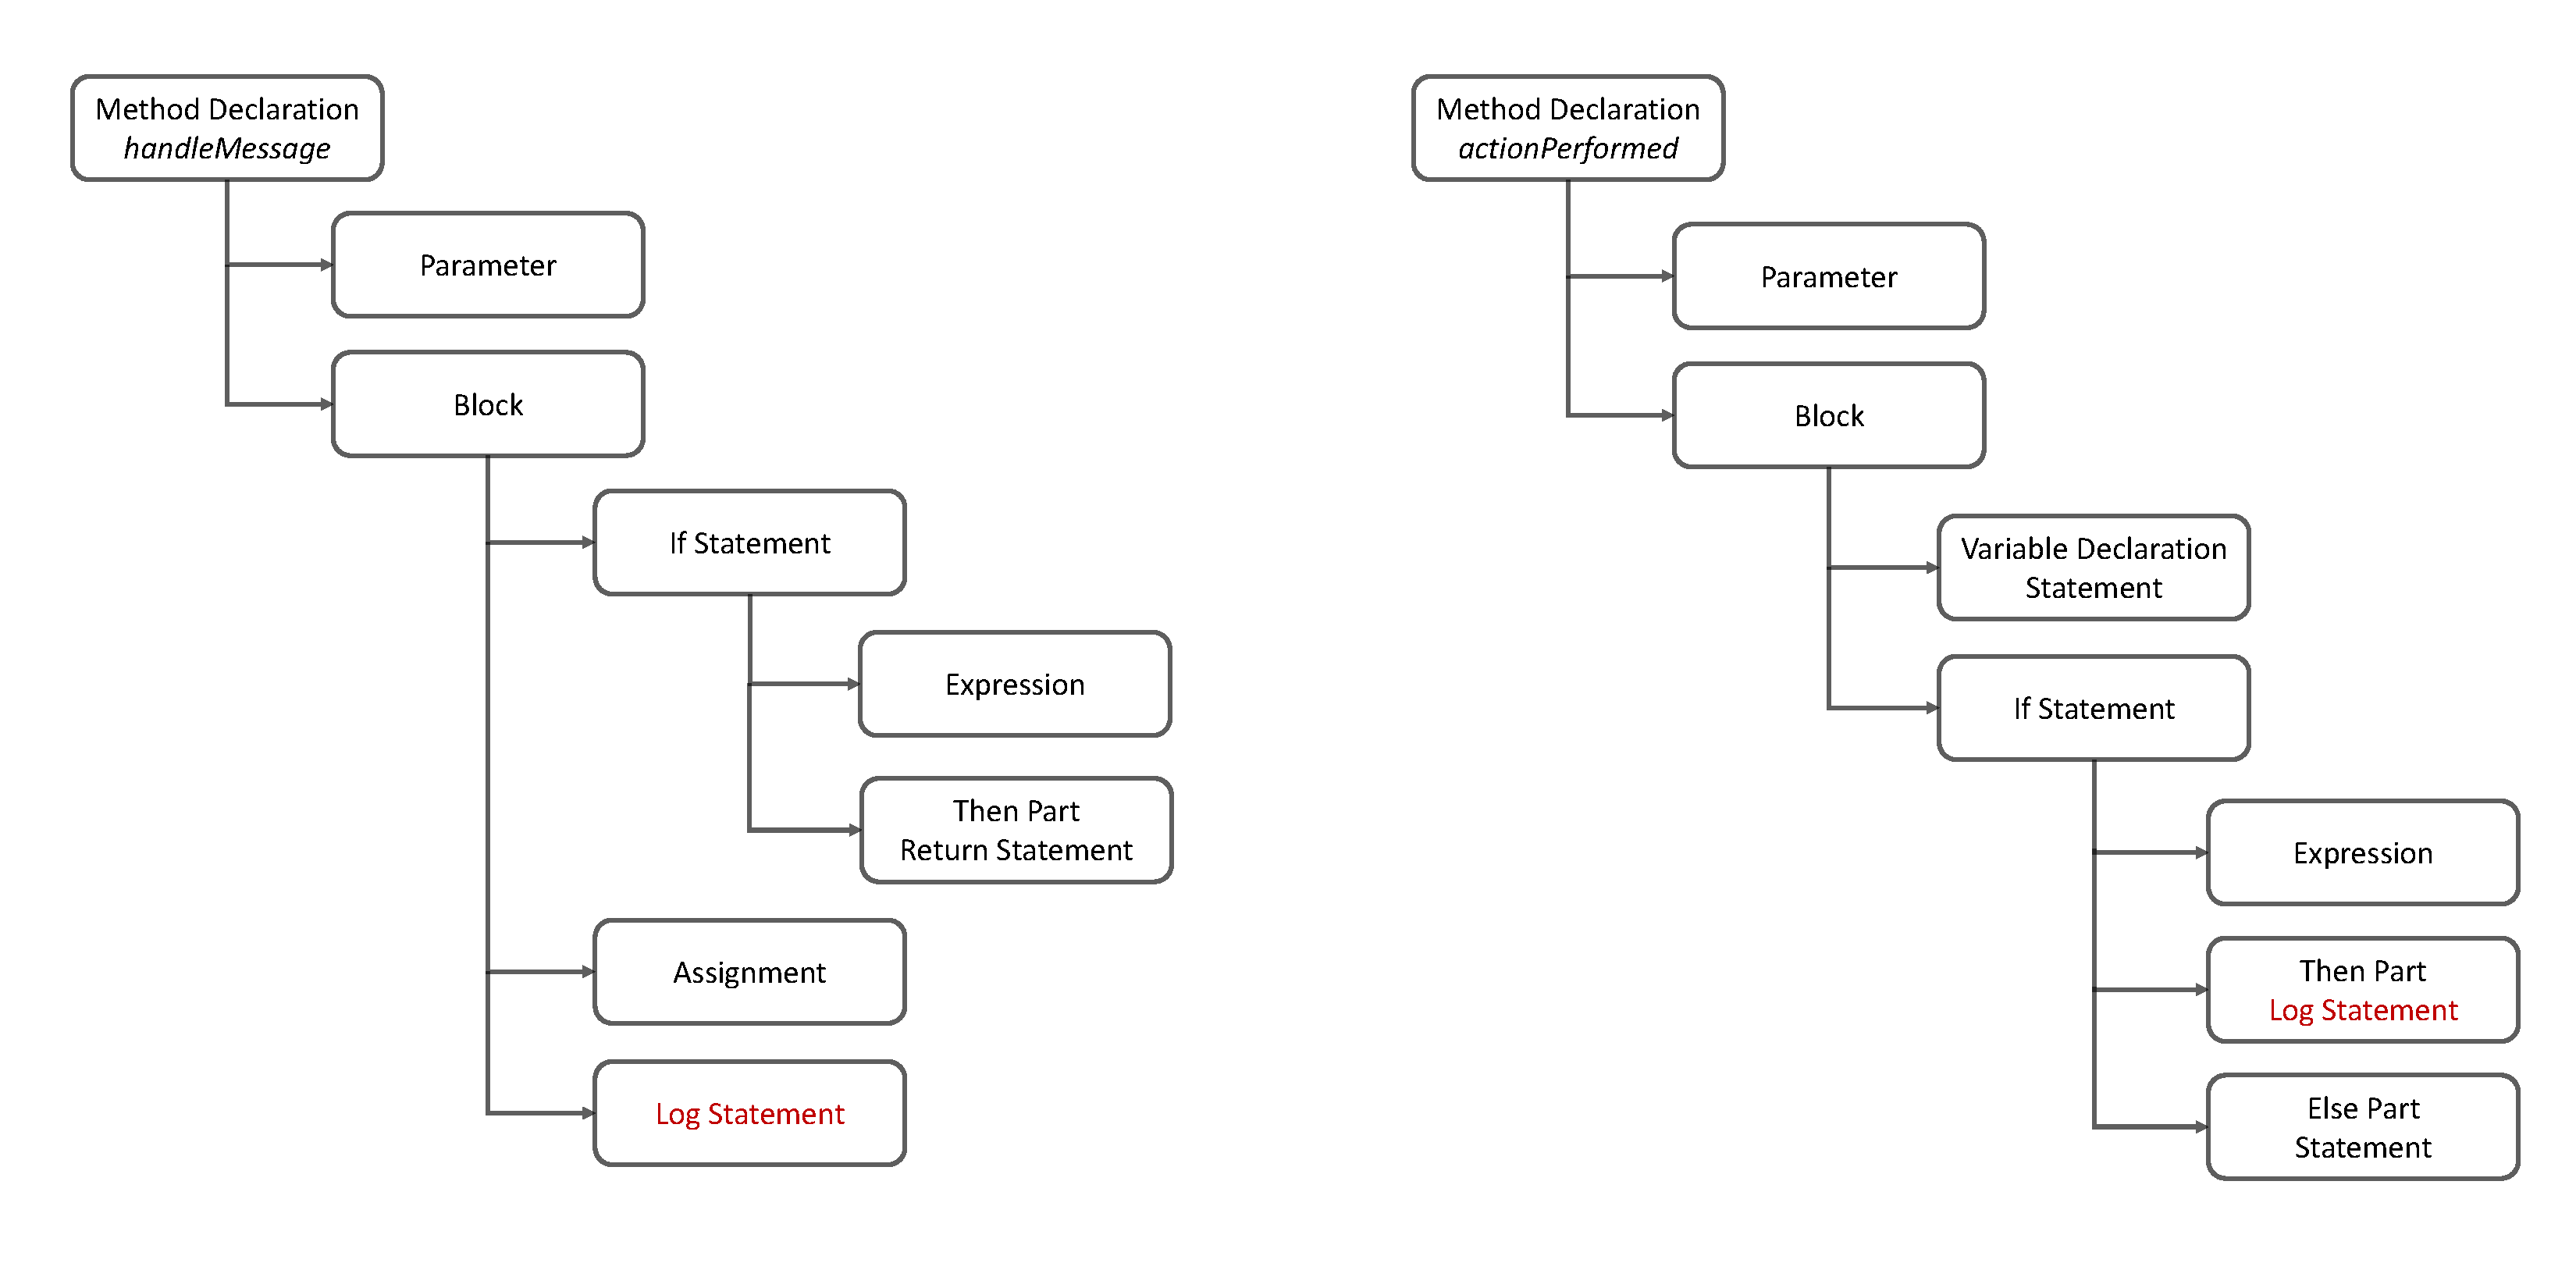
\includegraphics [width = \textwidth]{Drawing4/AST.pdf}
  \caption{Simple AST structure of examples in Figures~\ref{ch3-ex1} and~\ref{ch3-ex2}.}
  \label{fig:ast}
\end{figure}

In the JDT framework, structural properties of each AST node can be used to obtain specific information of the Java element it represents. These properties are stored in a map data structure that associates each property to its value and are divided into three types:
\begin{itemize} [leftmargin=0.7in]
\item \textit{Simple structural properties:} that contain a simple value which has a primitive or simple type or a basic AST constant (e.g., identifier property of a name node whose value is a String)
\item \textit{Child structural properties:} where the value is a single AST node (e.g., name property of a method declaration node)
\item \textit{Child list structural properties}: where the value is a list of child nodes (e.g., body declarations property of a class declaration node whose value is a list of body declaration nodes, including method declaration and field declaration nodes.)
\end{itemize}
%AST is made up of AST nodes as subtrees and simple values as leaves.
An instance of an AST structure can be represented in an abstract form that can be mapped to the definition of a term described in Section~\ref{AU}. As an example, the abstract form of ASTs of logging calls of Java classes in Figures~\ref{ch3-ex1} and~\ref{ch3-ex2} can be represented as:
\begin{itemize} [leftmargin=0.7in]
\item \textit{expression(expression(Log),name(log),arguments(leftoperand(message),+,\\rightoperand(" is empty"),qualifier(Log),name(WARNING)))}
\item \textit{expression(expression(Log),name(log),arguments(leftoperand(actionName),\\+,rightoperand("is an unknown action"),qualifier(Log),name(WARNING)))}
\end{itemize}

Where ASTNodes (e.g., \textit{expression, name,, qualifier}) might be viewed as function symbols and simple values (e.g., \textit{log, WARNING}) might be viewed as constants in the term definition. As described in Section~\ref{AU}, anti-unification utilizes variables that must be substituted with proper structures to re-create original structures. However, the AST structure does not contain any variables and so we need to construct an extended form of AST, which will be described in the following section.

% In order to map an instance of an AST to that form of structure, first we should understand how an AST structure holds its subtrees and leaves
%The goal of this phase is to construct an extension of the AST structure that would allow the creation of an anti-unified structure. 

\section{Constructing the AUAST} \label{AUAST}  
AUAST (Anti-unified AST) is an extended form of AST that allows the insertion of variables in place of any node in the tree structure, including both subtrees and leaves, to indicate variations between original structures. The AUAST addresses the limitations of AST to construct an anti-unifier by adding the following structural properties:
\begin{itemize} [leftmargin=.4in]
\item \textit{Simple Variable Property}: an extension of simple property referring to two simple values to allow the insertion of variables in place of leaves.
\end{itemize}
\begin{itemize} [leftmargin=.4in]
\item \textit{Child Variable Property}: an extension of child property referring to two child AST nodes to allow the insertion of variables in place of subtrees.
\end{itemize}
The anti-unification of AUASTs of logging calls in Figures~\ref{ch3-ex1} and~\ref{ch3-ex2} is depicted in Figure~\ref{fig:logging-anti}. The new variables \vars{X} and \vars{Y} are created to abstract away the structural variations. 
%\item it can be mapped to our recursive definition of a term, where AST nodes and simple values may be viewed as function-symbols and constants, respectively


\begin{figure} [H]
\[
\begin{tikzcd}[column sep=small] 
&  
{\makecell[l]{ expression(expression(Log),\\name(log),arguments(\\leftoperand(X),+,\\rightoperand(Y),\\qualifier(Log),\\name(WARNING)))}}
  \arrow{dr}{\ominus_2 = (X \rightarrow actionName, Y \rightarrow "is an unknown action")}
  \arrow[->,swap]{dl}{\ominus_1 = (X \rightarrow message, Y \rightarrow " is empty")} % <-- reflect the direction of the hook
\\
{\makecell[l]{expression(expression(Log),\\name(log),arguments(\\leftoperand(message),+,\\rightoperand(" is empty"),\\qualifier(Log),\\name(WARNING)))}}
&&
{\makecell[l]{
expression(expression(Log),\\name(log),arguments(\\leftoperand(actionName),\\+,rightoperand("is an unknown action"),\\qualifier(Log),\\name(WARNING))) }}
\end{tikzcd}
\]
  \caption{ The anti-unification of AUASTs of logging calls in the Examples 1 and 2.}
  \label{fig:logging-anti}
\end{figure}
%The AUASTs of log Method Invocation nodes from the Java classes in Figure~\ref{ch3-ex1} and Figure~\ref{ch3-ex2}.

Applying higher-order anti-unification on AUAST structures could help us in constructing a structural generalization by maintaining the common pieces and abstracting the differences away using variables. However, it is not comprehensive enough to solve our problem as it does not consider background knowledge about AST structures, such as syntactically different but semantically relevant structures, missing structures, and different ordering of arguments. In the following section, we will look at an extension of anti-unification, higher-order anti-unification modulo theories, and how it can sufficiently address the limitations of anti-unification in our context.


\section{Higher-order anti-unification modulo theories}   \label{HOAUMT}
%Anti-unification cannot incorporate any background knowledge such as sematic knowledge required to solve our problem, and we should apply an extended form of anti-unification, called higher-order anti-unification modulo theories, where a set of equivalence equations is defined to incorporate semantic knowledge of structural equivalences supported by the Java language specification. An equivalence equation $=_E$ determines which terms are considered equal, and the set of equivalence equations must be applied on higher-order extended structures to allow the anti-unification of AST structures that are not identical but are semantically equivalent.
In higher-order anti-unification modulo theories, a set of equivalence equations is defined to incorporate background knowledge. Each equivalence equation $=_E$ determines which terms are considered equal and a set of these equations can be applied on higher-order extended structures to determine structural equivalences. For example, we have introduced an equivalence equation $=_E$, such that F(X,Y) $=_E$ F(Y,X) to indicate that the ordering of arguments does not matter in our context.

% nil restriction!!!!
We have also introduced a theory, called NIL- theory, that adds the concept of NIL structure, which is defined to create a structure out of nothing, and defines an equivalence equation $=_E$ for it. The NIL structure can be used to anti-unify two structures when a substructure exists in one but is missing from the other. However, some requirements should be taken to avoid the overuse of NIL structures such that the original structures must have common substructures but vary in the size for dissimilar substructures. For example, we can anti-unify the two structures \vars{b} and \vars{f(a,b)} through the application of NIL-theory by creating the term \vars{nil(nil,b)} which is $=_E$ to \vars{f(b)} and anti-unifying \vars{nil(nil,b)} with \vars{f(a,b)} as depicted in Figure~\ref{fig:anti-nil}.
% to introduce an equivalence equation =E for the NIL structure
% it should be modified
% should it be different?
\begin{figure} [H]
\[
\begin{tikzcd}[column sep=small] 
&  
  X(Y,b)
  \arrow{dr}{\ominus_2 = ( X \rightarrow nil, Y \rightarrow nil) }
  \arrow[->,swap]{dl}{\ominus_1 = ( X \rightarrow f, Y \rightarrow a)} % <-- reflect the direction of the hook
\\
f(a,b)
&&
nil(nil,b) =_E  b 
\end{tikzcd}
\]
  \caption{ The anti-unification of the terms f(a, b) and nil(nil,b).}
  \label{fig:anti-nil}
\end{figure}


We have also defined a set of equivalence equations to incorporate semantic knowledge of structural equivalences supported by the Java language specification as it provides various ways to define the same language specifications. These theories should be applies on higher-order extended structures to anti-unify AST structures that are not identical but are semantically equivalent. For example, consider for- and while- statements that are two types of looping structure in Java programming language that have different syntax but semantically cover the same concept. Let us look at the \vars{$for(i=0;i<10;i++)$} and \vars{$while(i<10)$} code snippets, whose AST structures can be represented as \vars{$for(initializer(i,=,0),expression(i,<,10), updaters(i,++))$} and \vars{$while(expression(i,<,10))$}, respectively. We could define an equivalence equation $=_E$ that allows the anti-unification of for- and while- statements which are semantically similar structures. We also need to utilize the NIL-theory to handle varying number of arguments as the for- loop has three arguments whereas the while- loop has one. Using the NIL-theory we can create the structure \vars{$while(nil(nil,nil,nil),expression(i,<,10), nil(nil,nil))$} that is $=_E$ to \vars{$while(expression(i,<,10))$} and construct the anti-unifier, \vars{$V_0(V_1(V_2,V_3,V_4),expression(i,<,10), V_5(V_2,V_6))$} as depicted in Figure~\ref{fig:for-while}.

\begin{figure} [H]
\[
\begin{tikzcd}[column sep=small] 
&  
  \makecell[l]{V_0(V_1(V_2,V_3,V_4),\\expression(i,<,10),\\ V_5(V_2,V_6)) }
  \arrow{dr}{\ominus_2 = \makecell[l]{ V_0 \rightarrow while, V_1 \rightarrow nil,\\ V_2 \rightarrow nil, V_3 \rightarrow nil,\\ V_4 \rightarrow nil, V_5 \rightarrow nil, V_6 \rightarrow nil} }
  \arrow[->,swap]{dl}{\ominus_1 = \makecell[l]{V_0 \rightarrow for, V_1 \rightarrow initializer, \\V_2 \rightarrow i, V_3 \rightarrow =, V_4 \rightarrow 0, \\V_5 \rightarrow updaters, V_6 \rightarrow ++ }} % <-- reflect the direction of the hook
\\
  \makecell[l]{for(initializer(i,=,0),\\expression(i,<,10),\\ updaters(i,++))} 
&&
  \makecell[l]{while(nil(nil,nil,nil),\\expression(i,<,10),\\ nil(nil,nil)) } 
\end{tikzcd}
\]
  \  \caption{ The anti-unification of the structures \vars{$for(initializer(i,=,0),expression(i,<,10), updater(i,++))$} and \vars{$while(nil(nil,nil,nil),expression(i,<,10), nil(nil,nil))$}.}
  \label{fig:for-while}
\end{figure}
% higher-order extension and the equational theories
% provide a better example
However, defining complex substitutions in higher-order anti-unification modulo theories results in losing the uniqueness of MSA. For example, consider the terms \vars{$f(g(a,e))$} and \vars{$f(g(a,b),g(d,e))$}. As described in Figure~\ref{fig:multipleMSA}, two MSAs exist for these terms: we can anti-unify \vars{$g(a,e)$} and \vars{$g(a,b)$} to create the anti-unifier \vars{$g(a,X_0)$} and anti-unify \vars{$g(d,e)$} with the NIL structure to create the anti-unifier \vars{$Y(Z,X_1)$}; or we can anti-unify \vars{$g(a,e)$} and \vars{$g(d,e)$} to create the anti-unifier \vars{$g(X_0,e)$} and anti-unify \vars{$g(a,b)$} with the NIL structure to create the anti-unifier \vars{$Y(Z,X_1)$}.

\begin{figure} [H]
\[
\begin{tikzcd}[column sep=small] 
&  
  f(g(X_0,e),Y(Z,X_1))
  \arrow{dr}{\ominus_2 = ( X_0 \rightarrow a, Y \rightarrow nil, Z \rightarrow nil, X_1 \rightarrow nil) }
  \arrow[->,swap]{dl}{\ominus_1 = ( X_0 \rightarrow d, Y \rightarrow g, Z \rightarrow a, X_1 \rightarrow b)} % <-- reflect the direction of the hook
\\
f(g(a,b), g(d,e))
&&
f(g(a,e)) 
\end{tikzcd}
\]	

\[
\begin{tikzcd}[column sep=small] 
&  
  f(g(a,X_0),Y(Z,X_1))
  \arrow{dr}{\ominus_2 = ( X_0 \rightarrow e, Y \rightarrow nil, Z \rightarrow nil, X_1 \rightarrow nil) }
  \arrow[->,swap]{dl}{\ominus_1 = ( X_0 \rightarrow b, Y \rightarrow g, Z \rightarrow d, X_1 \rightarrow e)} % <-- reflect the direction of the hook
\\
f(g(a,b), g(d,e))
&&
f(g(a,e)) 
\end{tikzcd}
\]
  \caption{The anti-unification of the terms \vars{f(g(a,b), g(d,e))}
and \vars{f(g(a,e))} that creates multiple MSAs.}
  \label{fig:multipleMSA}
\end{figure}


Despite having multiple potential MSAs, we need to determine one single MSA that is the most appropriate in our context. However, the complexity of finding an optimal MSA is undecidable in general [Cottrell et al., 2008] since an infinite number of possible substitutions can be applied on every variable. Therefore, we need to use an approximation technique to construct one of the best MSAs that can sufficiently solve our problem.
% reason since?
%Our goal is to find an MSA that is an approximation of the best fit to our application


\section{The Jigsaw framework}  \label{Jigsaw}
The Jigsaw tool is developed by Cottrell et al. [2008] to determine the structural correspondences between two Java source code fragments through the application of higher-order anti-unification modulo theories such that one fragment can be integrated to the other one for small scale code reuse. Jigsaw could help us to determine potential candidate structural correspondences between AST nodes of logged Java classes by producing an augmented form of AST, called CAST (Correspondence AST), where each node holds a list of candidate correspondence connections between the two structures, each representing an anti-unifier. It also develops a measure of similarity to indicate how similar the nodes involved in each correspondence connection are. The Jigsaw similarity function relies on structural correspondence along with a simple knowledge of semantic equivalences supported by the Java language specification, and it returns a value between 0 and 1 that indicates zero and total structural matching, respectively. In addition, several semantical heuristics are used to improve the accuracy of similarity measurement by allowing the comparison of AST nodes that are not syntactically identical but are semantically related to each other.

As an example, the similarity between names of AST nodes is measured using a normalized computation based on the length of longest common substring. Another example is the comparison of \vars{int} and \vars{long} variable types, where an arbitrary value of 0.5 is defined as the similarity value as they are not syntactically identical but are not semantically unrelated. In addition, the Jigsaw framework also detects the structural correspondence between  for-, enhanced-for-, while-, and do- loop statements; and if- and switch- conditional statements. As an example, Figure~\ref{fig:meth-ast-1} shows the structural correspondence connections created by Jigsaw between the AST nodes of Examples 1 and 2 along with the similarity value for each correspondence connection.

\begin{figure} [H]
  \centering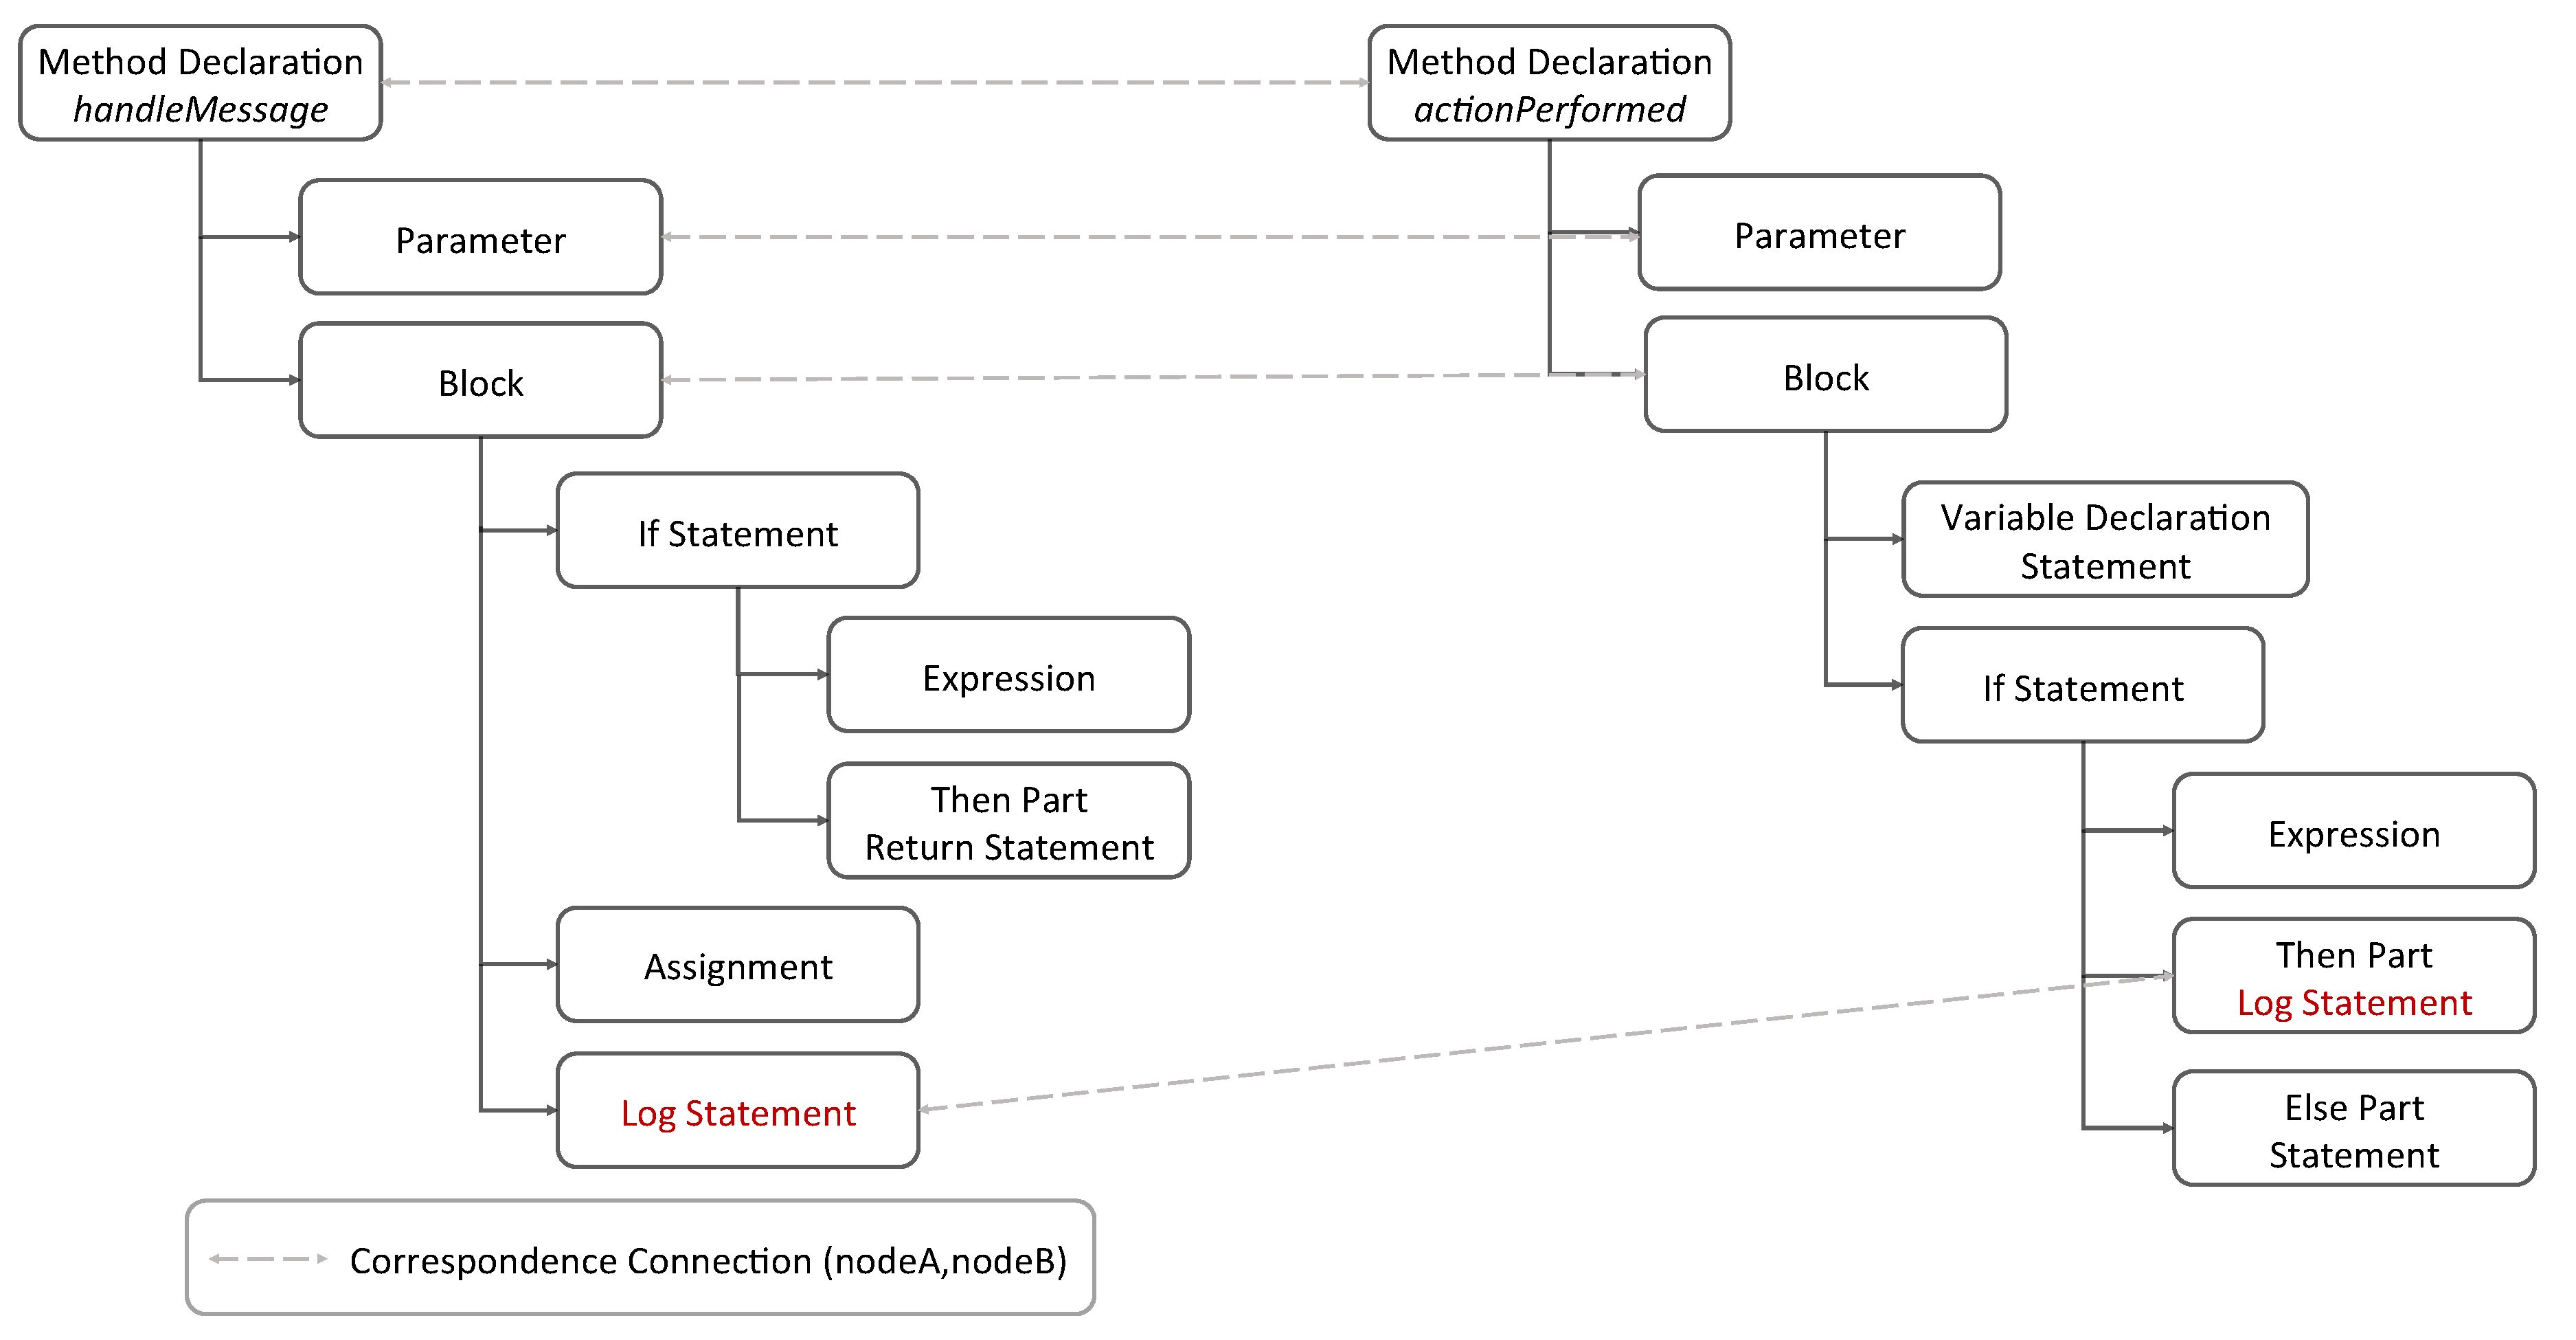
\includegraphics [width = \textwidth]{Drawing4/FirstCorr.pdf}
  \caption{Simple CAST structure of examples in Figures~\ref{ch3-ex1} and~\ref{ch3-ex2}. The links between AST nodes indicate structural correspondence connections created by the Jigsaw framework along with the similarity value.}
  \label{fig:meth-ast-1}
\end{figure}

However, the Jigsaw tool does not suffice to construct an anti-unifier that is the best fit to our application. In addition, the Jigsaw similarity function does not measure the similarity of two logged Java classes with a focus on logging calls, which is needed in our context. To address these issues, we should develop a greedy selection algorithm to approximate the best anti-unifier by determining the best correspondence for each node. In the following chapter, we will discuss our approach to construct structural generalizations and our implementation by means of the higher-order anti-unification modulo theories and the Jigsaw framework.

 
\section{Summary}  \label{summary}
In this chapter, we described anti-unification as a technique to construct a common generalization of two given terms. We have also introduced an extended form of anti-unification, which is called higher-order anti-unification modulo theories, where a set of equivalence equations can be applied on higher-order extended structures to incorporate background knowledge. In addition,
we provided a brief description of AST that maps Java source code in a tree structure form, and why an extended form of it, named AUAST, is required to create higher-order structures specific to our problem context. Finally, we discuss the Jigsaw framework and how it could assist us in determining the potential structural correspondences. 
